\section{Silicon --- Boltzmann transport}
\label{sec16:SiBZT}

\begin{itemize}
	\item Outline: {\it Obtain MLWFs for the valence and low-lying conduction states of Si. Calculate the electrical conductivity, the Seebeck coefficient and the thermal conductivity in the constant relaxation time approximation using the {\tt BoltzWann} module.}
\end{itemize}

\begin{figure}[h!]
\centering
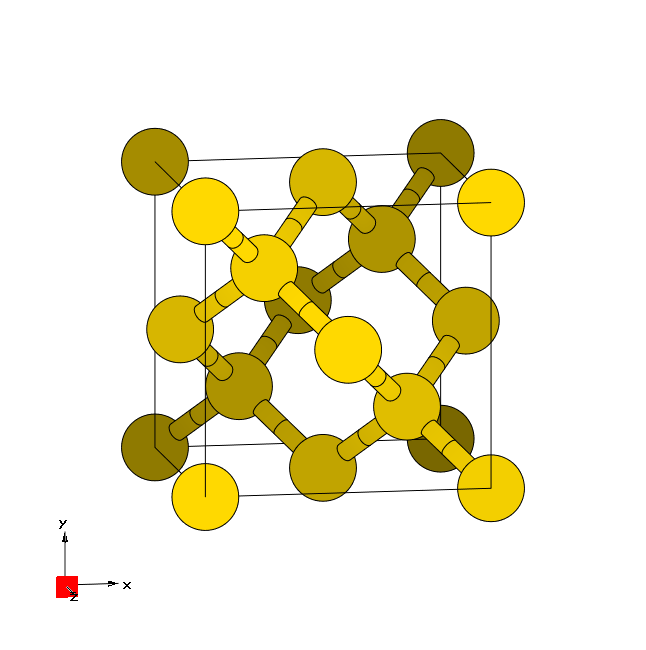
\includegraphics[width=0.25\columnwidth,trim={45pt 45pt 55pt 55pt},clip]{figure/example11/silicon.png}
\caption{Unit cell of Silicon crystal plotted with the \xcrysden{} program.}
\label{fig16.0}
\end{figure}

\begin{itemize}
	\item[1-5] For this example we are only going to show the solutions from point 6 onwards, as the first 5 steps are the usual steps to obtain MLWFs.
	\item[6] {\it Run {\tt postw90} to calculate the transport coefficients.}
	\item {\it Inspect the output file {\tt Si.wpout}. Check if no warnings are issued. Note that if no special flags are passed to {\sc BoltzWann}, it assumes that the {\it ab initio} calculation did not include magnetization effects, and thus it sets to 2 the number of electrons per state.}

Below the section in the {\tt Si.wpout} relative to the Boltzmann transport, where it reports the number of electrons per state and the relaxation time in fs.
\end{itemize}
\begin{tcolorbox}[sharp corners,boxrule=0.5pt]
{\small
\begin{verbatim}
 *---------------------------------------------------------------------------*
 |                   Boltzmann Transport (BoltzWann module)                  |
 *---------------------------------------------------------------------------*
 | Please cite the following paper when publishing results obtained using    |
 | the BoltzWann module:                                                     |
 | G. Pizzi, D. Volja, B. Kozinsky, M. Fornari, and N. Marzari,              |
 | Comp. Phys. Comm. 185, 422 (2014); DOI:10.1016/j.cpc.2013.09.015          |
 *---------------------------------------------------------------------------*

   Calculating Transport Distribution function (TDF) and DOS...
     k-grid used for band interpolation in BoltzWann: 40x40x40
     Number of electrons per state: 2
     Relaxation time (fs):    10.00000000     
   TDF and DOS calculated.

   Transport properties calculated.

 *---------------------------------------------------------------------------*
 |                        End of the BoltzWann module                        |
 *---------------------------------------------------------------------------*
\end{verbatim}
}
\end{tcolorbox}  


{\it Using your favourite plotting program, plot the {\tt Si\_boltzdos.dat} file to inspect the DOS.}

Plot shown in \Fig{fig16.1}-(a).


{\it Using your favourite plotting program, plot columns 1 and 3 of the {\tt Si\_seebeck.dat} file to inspect the
$S_{xx}$ component of the Seebeck coefficient as a function of the chemical potential $\mu$, at $T = 300$ K.}

Plot shown in \Fig{fig16.1}-(b).

\begin{figure}[h!]
\centering
\subfloat[]{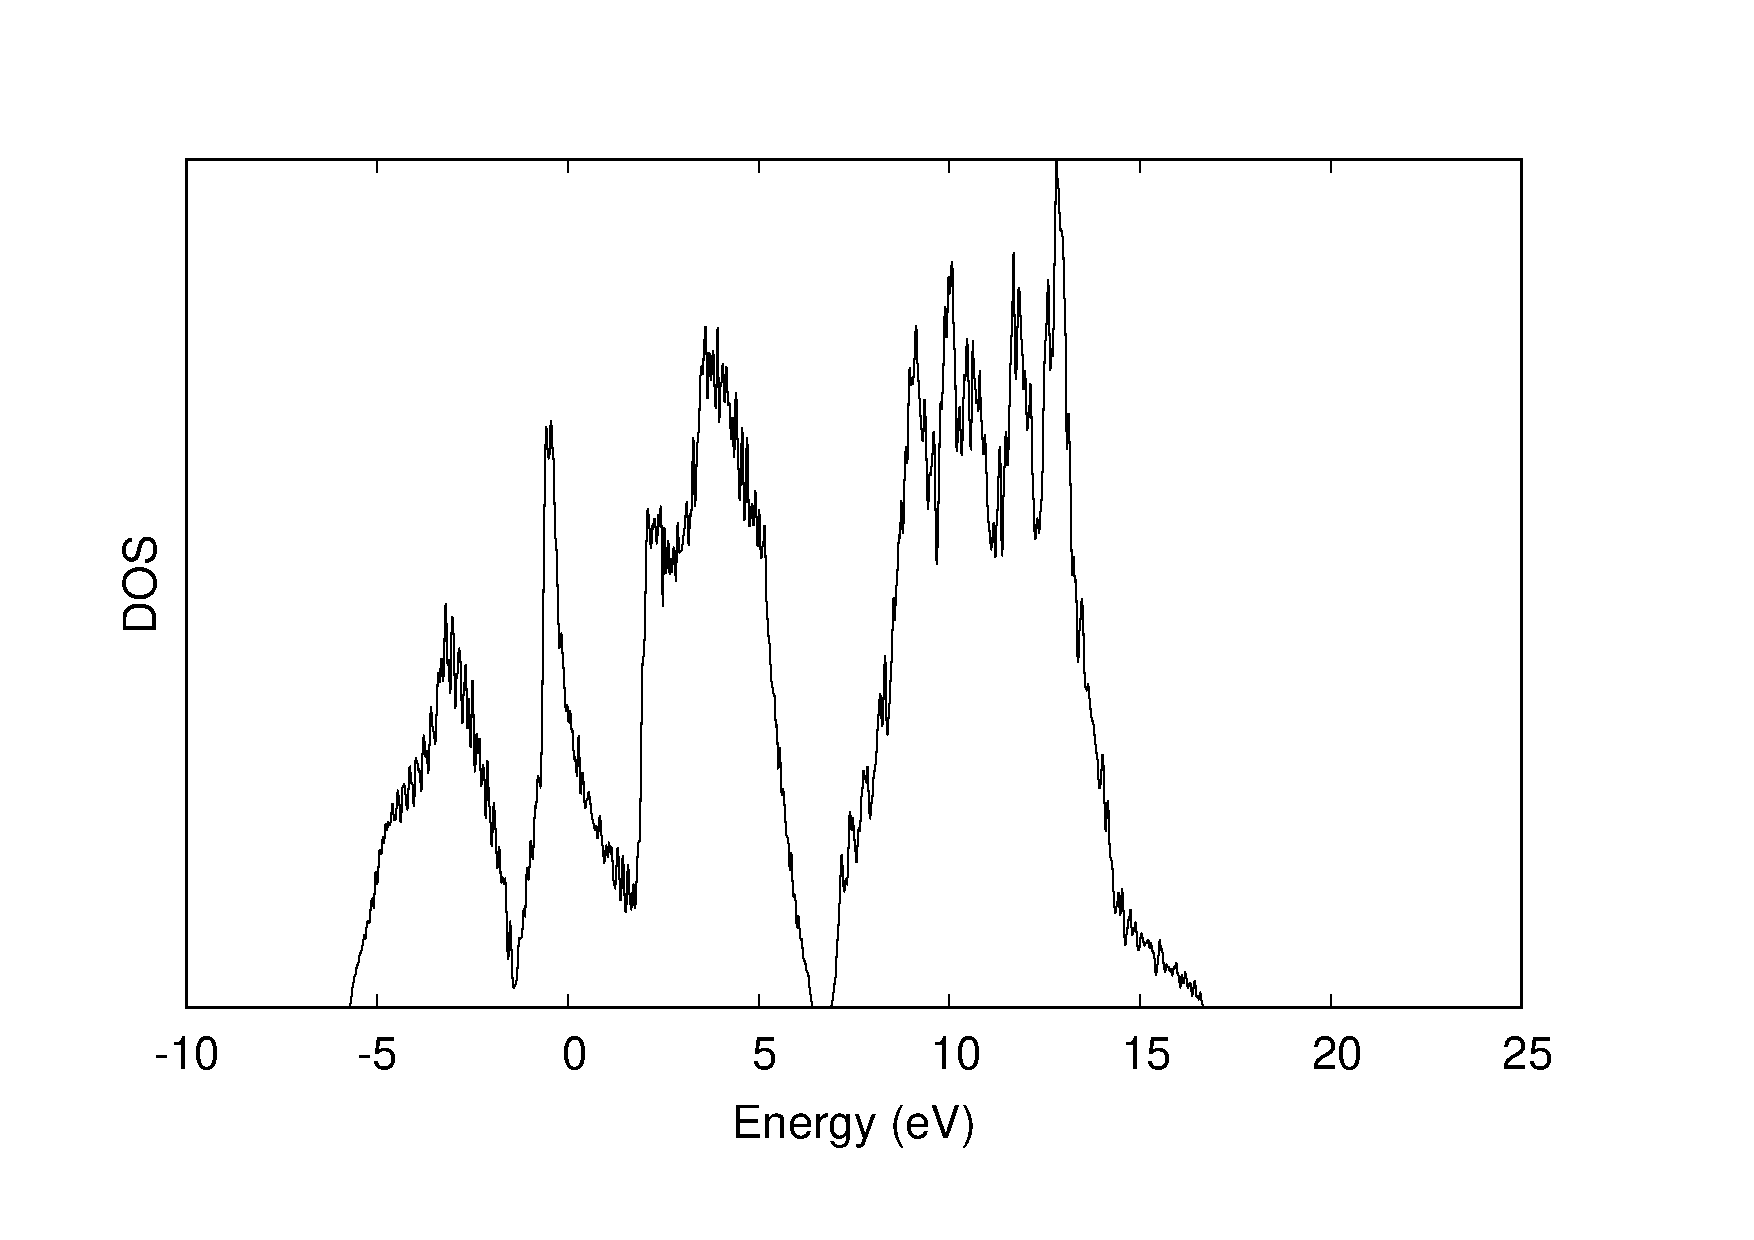
\includegraphics[width=0.5\columnwidth,trim={30pt 30pt 50pt 50pt},clip]{figure/example16/Si_boltzdos.pdf}}
\centering
\subfloat[]{
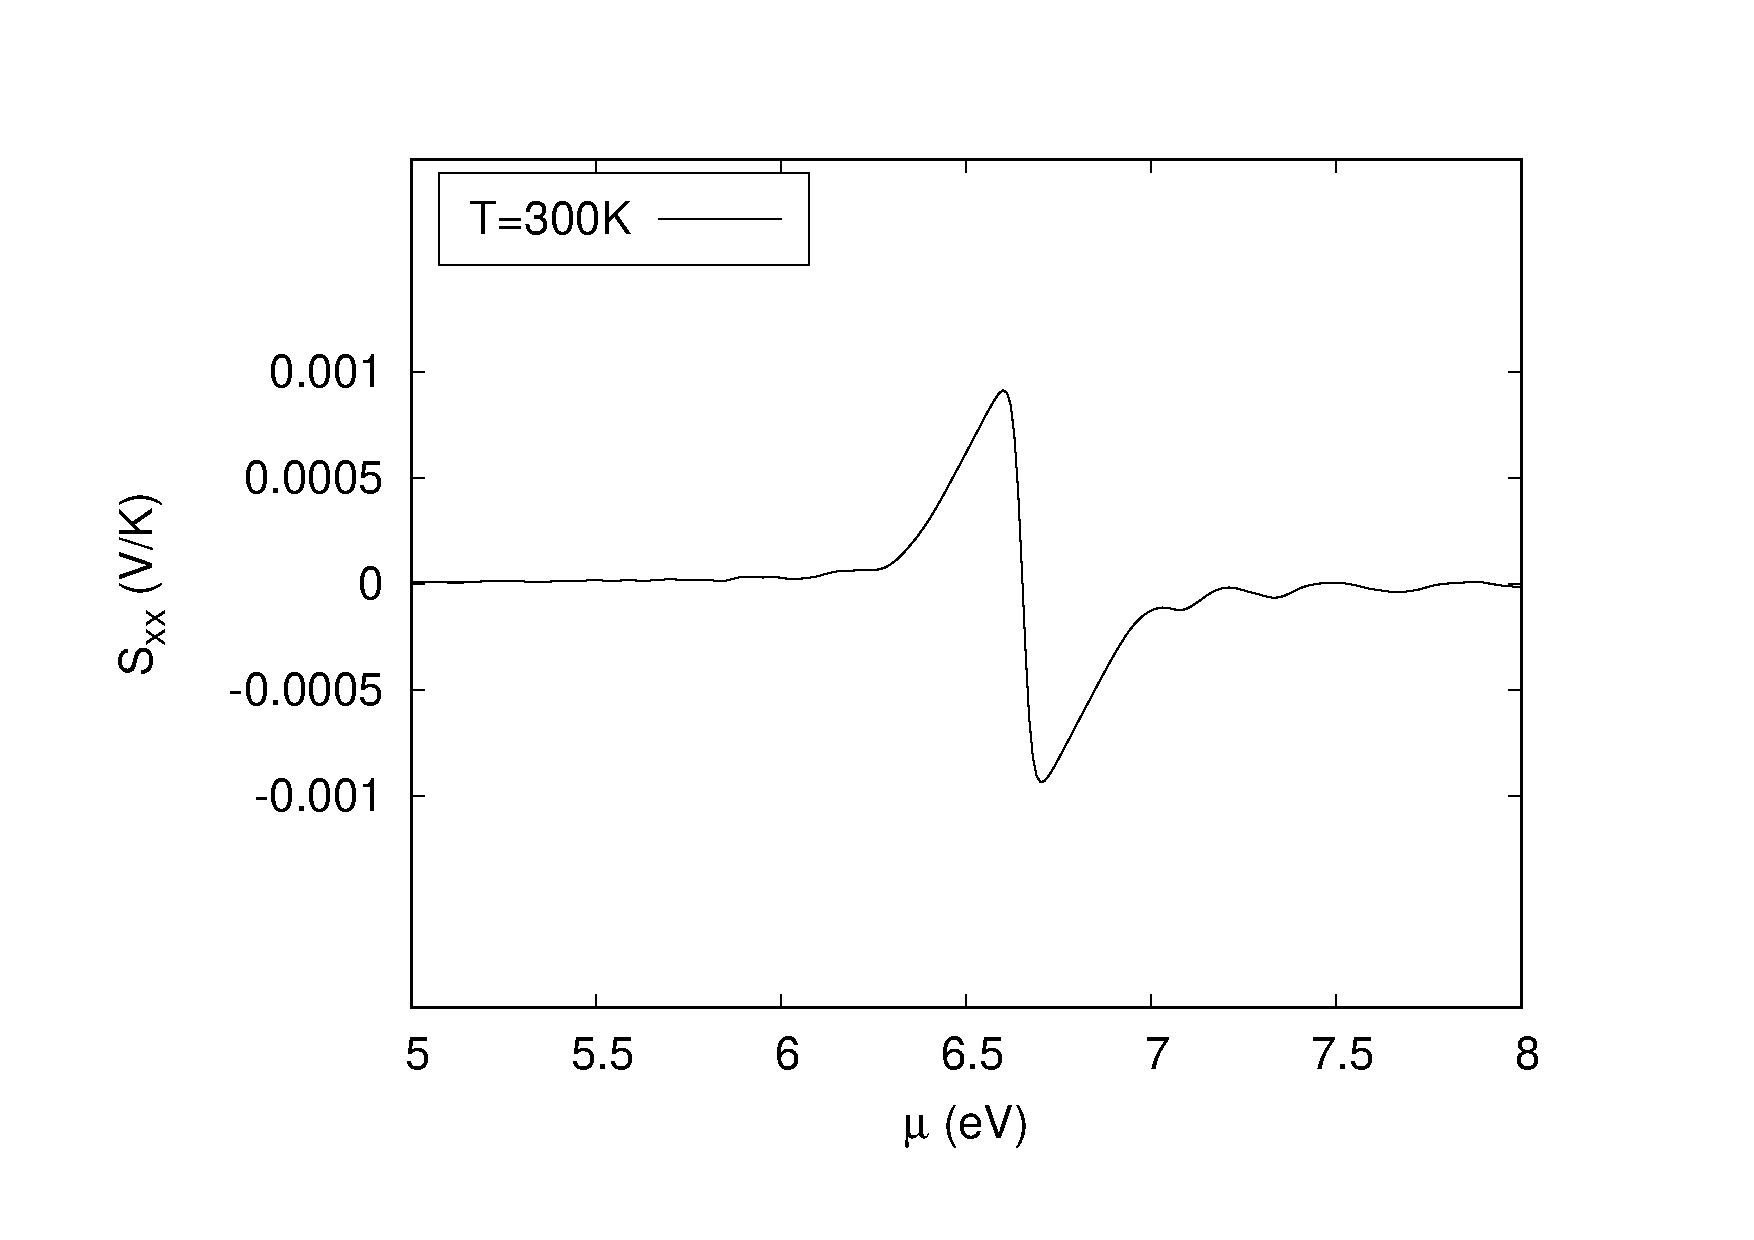
\includegraphics[width=0.5\columnwidth,trim={30pt 30pt 50pt 50pt},clip]{figure/example16/Si_seebeck.pdf}}
\caption{Panel (a) DOS of Silicon computed with {\sc BoltzWann}. Panel (b) $S_xx$ component of the Seebeck tensor as function of the chemical potential $\mu$ computed with {\sc BoltzWann} at $T = 300$ K.}\label{fig16.1}
\end{figure}


\subsection*{Further ideas}
\begin{itemize}
  \item {\it Change the interpolation to a $60\times60\times60$ mesh and run again postw90 to check if the results
for the transport properties are converged.}

Plot of the two DOS with $40\times40\times40$ (red line) and $60\times60\times60$ (blue line) are shown in \Fig{fig16.3}. We can see that all the peaks for the valence and conduction states in the $60\times60\times60$ DOS are also reproduced in the $40\times40\times40$ DOS (even though there is some noise, which however does not affect the qualitative description.)

\begin{figure}[h!]
\centering
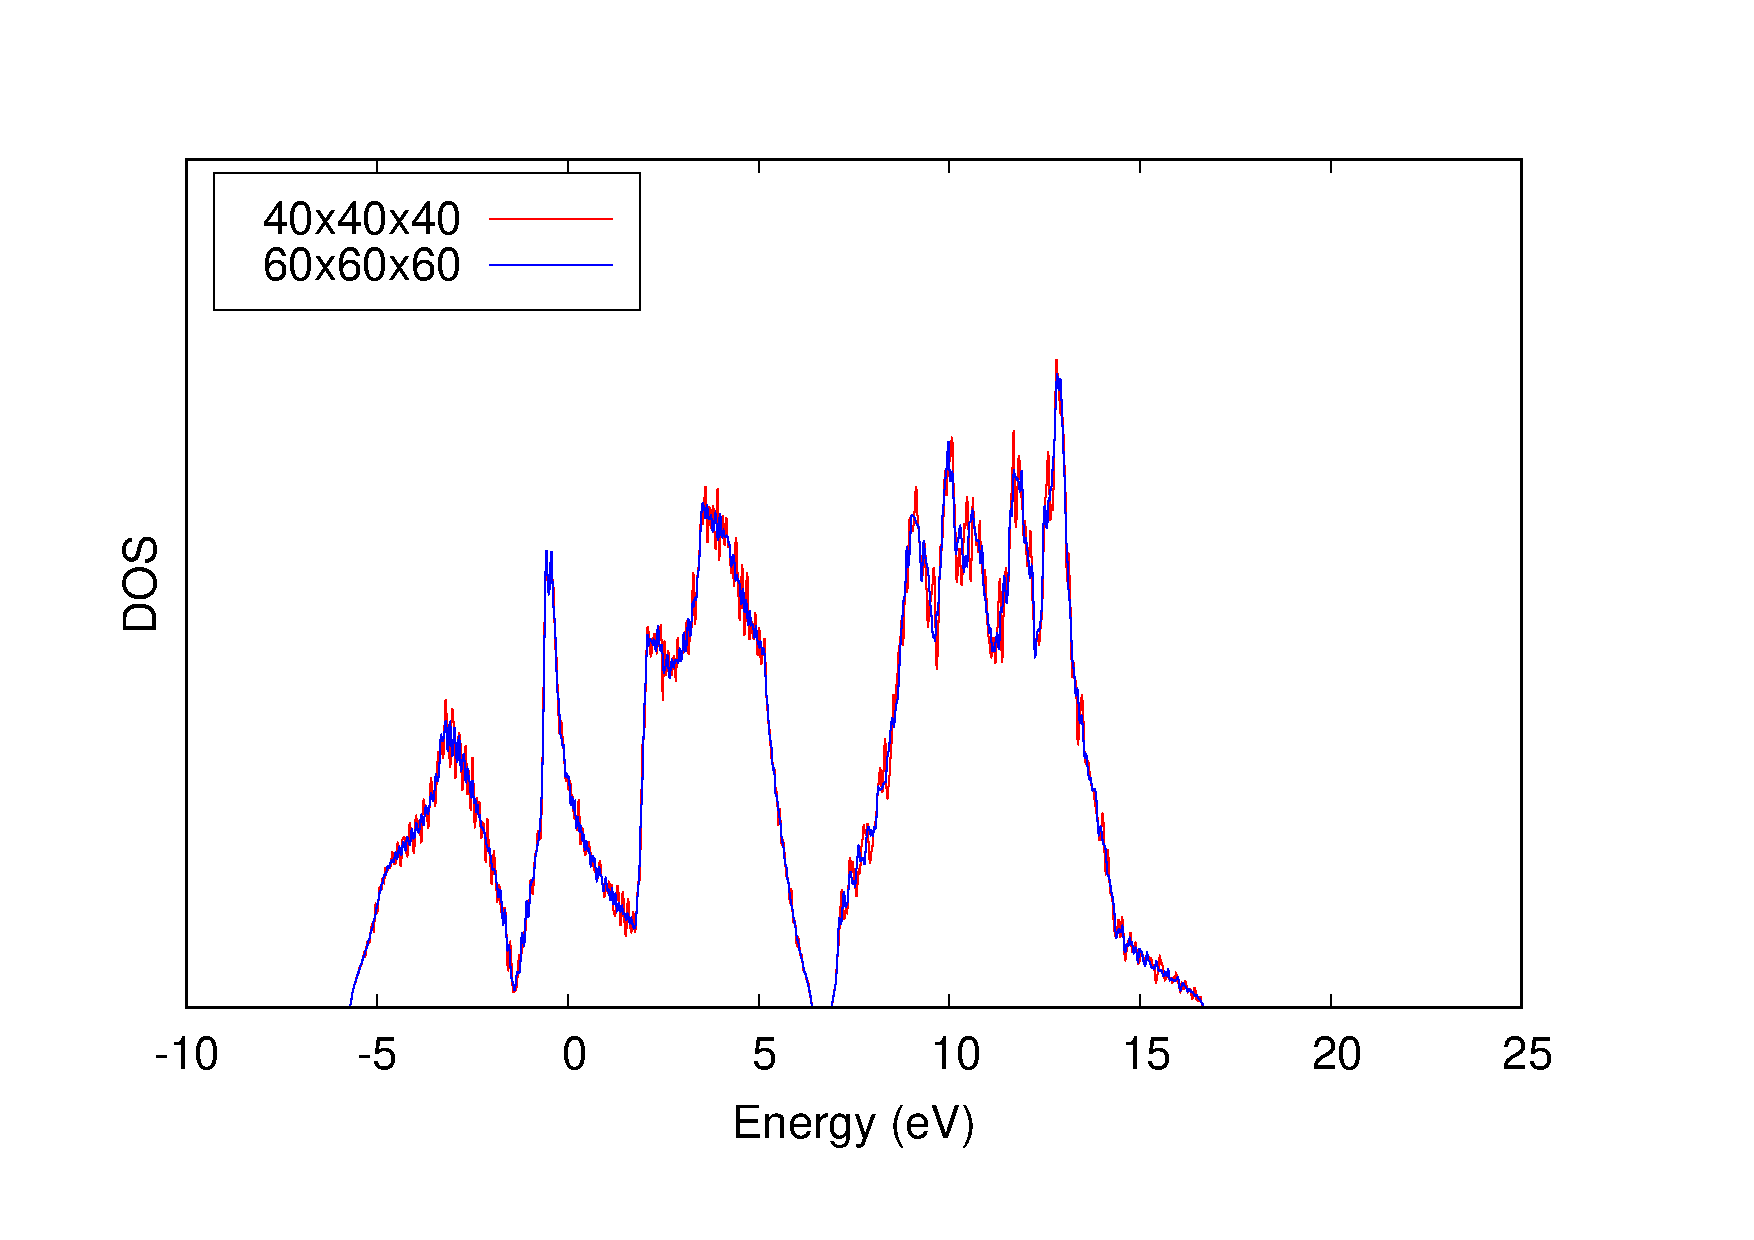
\includegraphics[width=0.7\columnwidth]{figure/example16/Si_boltzdos_convergence.pdf}
\caption{Convergence of DOS}\label{fig16.3}
\end{figure}

  \item {\it Change the {\tt Si.win} input file so that it calculates the transport coefficients for temperatures from
$300$ to $700$ K, with steps of $200$ K. Rerun {\tt postw90} and verify that the increase in execution time
is negligible (in fact, most of the time is spent to interpolate the band structure on the k mesh).
Plot the Seebeck coefficient for the three temperatures $T = 300$ K, $T = 500$ K and $T = 700$ K.
To do this, you have to filter the {\tt Si\_seebeck.dat} to select only those lines where the second
column is equal to the required temperature. A possible script to select the $S_{xx}$ component of the
Seebeck coefficient for $T = 500$ K using the {\tt awk/gawk} command line program is the following:
{\tt 
\begin{quote}
awk '{if (\$2 == 500) {print \$1, \$3;}}' < Si\_seebeck.dat > Si\_seebeck\_xx\_500K.dat
\end{quote}}
}

Below is shown the total wall-time for the two calculations done with the original set up, \ie{} $T_{min} = T_{max} = 300$ K and $T_{min} = 300$ K, $T_{max} = 700$ K, $\Delta T = 200$ K.

\begin{tcolorbox}[sharp corners,boxrule=0.5pt]
{\small
\begin{verbatim}
 Total Execution Time          16.356 (sec)
\end{verbatim}
}
\end{tcolorbox}

\begin{tcolorbox}[sharp corners,boxrule=0.5pt]
{\small
\begin{verbatim}
 Total Execution Time          16.108 (sec)
\end{verbatim}
}
\end{tcolorbox}

The plot of $S_{xx}(\mu)$ for different values of $T$ is shown in \Fig{fig16.4}

\begin{figure}[h!]
\centering
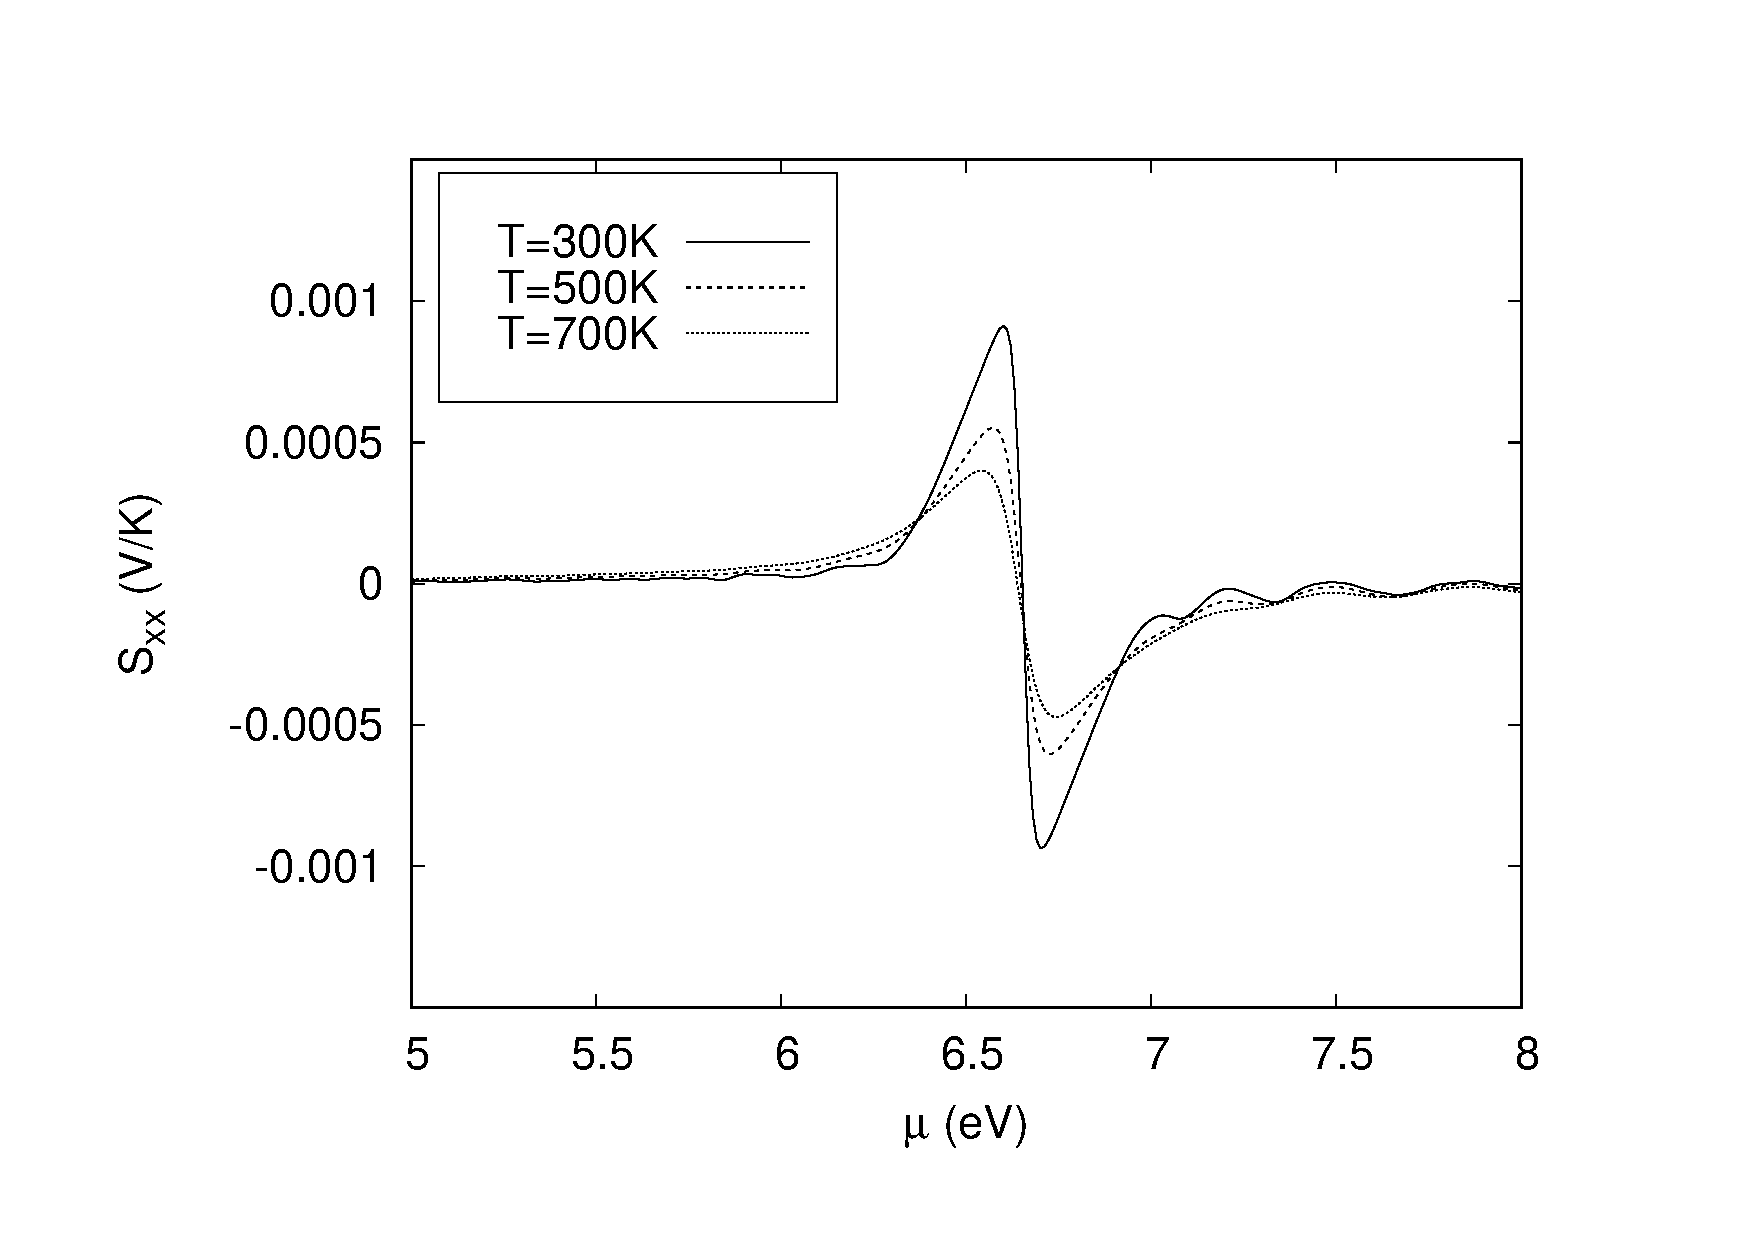
\includegraphics[width=0.7\columnwidth]{figure/example16/Si_seebeck_T.pdf}
\caption{$S_{xx}$ component of the Seebeck tensor as function of the chemical potential $\mu$ for different values of the temperature: $T = 300$ K (solid purple), $T = 500$ K (solid green) and $T = 700$ K (solid blue).}\label{fig16.4}
\end{figure}

\item {\it Try to calculate the Seebeck coefficient as a function of the temperature, for a n--doped sample
with, e.g., $n = 10^{18}$ cm$^{-3}$. Note that to this aim, you need to calculate consistently the value
$\mu(T)$ of the chemical potential as a function of the temperature, so as to reproduce the given value
of $n$. Then, you have to write a small program/script to interpolate the output of {\sc BoltzWann},
that you should have run on a suitable grid of $(\mu,T)$ points.}

ASSUMPTIONS: 1) The addition of a $n-$type dopant does not modify the electronic structure, it only moves the Fermi level up; 2) The density of states is temperature-independent. $\mu(T)$ is a decreasing monotonic function of $T$.

To obtain a $\mu(T)$ in a consistent way we use the above assumptions and the following equation:
\begin{equation}
N_c + N_v = \int_{-\infty}^{+\infty}\! \mathrm{d}\varepsilon \, g(\varepsilon,T=0)\,f(\varepsilon,\mu(T)),\label{eq16.1}
\end{equation}
where $N_v=8$, number of valence electrons per unit cell when no dopants are considered, $N_c= nV_{cell}$ is the number of carriers per unit cell ($V_{cell}$ is the volume of the unit cell in cm$^{-3}$). $g(\varepsilon,T=0)$ is the density of states at $T=0$K and by assumption it does not change with $T$. Finally, $f(\varepsilon,\mu(T))$ is the Fermi-Dirac distribution as a function of $\varepsilon$ and $T$
\begin{equation}
f(\varepsilon,\mu(T)) = \frac{1}{1 + \exp[\frac{\varepsilon - \mu(T)}{\kappa_B T}]}
\end{equation}
For each $T$ we find the value of the $\mu(T)$ such as the integral is (approximately) $N_c + N_v$. % MATLAB code used to generate $\mu(T)$ and the script to produce the graph. 
\footnote{\footnotesize{This can be easily achieved with any code, \eg{} Python, MATLAB or even bash.}}
The values of $\mu$ for $T$ in the range [300 K--700 K] are shown in \Tab{tab16.1}
\begin{table}
\centering
\captionsetup{width=.5\textwidth}
\caption{Values of the chemical potential $\mu$ in eV as a function of $T$ in K, computed by numerically solving Eq.~\ref{eq16.1}.}
\begin{tabular}{@{} cc @{}}\toprule[1.5pt]
$T$ [K] & $\mu$ [eV] \\\midrule
300 & 6.839 \\
400 & 6.798 \\
500 & 6.752 \\
600 & 6.707 \\
700 & 6.677 \\\bottomrule[1pt]
\end{tabular}\label{tab16.1}
\end{table} 

In practice we do not perform an interpolation but we run a single calculation with $\Delta \mu = 0.001$ eV since these are not expensive and then we filter out the result from {\tt Si\_seebeck.dat} with the following simple script
{\tt
\begin{quote}
mulist=`cat mu.dat | awk '{printf "i4" \$1}'`; i=0; for mu in \$mulist; do i=`echo \$i+1|bc` ; cat Si\_seebeck.dat | awk -v "mu=\$mu" '{if(\$1==mu) print \$1,\$2,\$3,\$7,\$11}' | awk -v "Tcol=\$i" '{if(NR==Tcol) print \$1, \$2, \$3, \$4, \$5}' >> Si\_seebeck\_vs\_T.dat;done
\end{quote}
}
where {\tt mu.dat} is a data file containing the second column of \Tab{tab16.1}. \Fig{fig16.5} shows the plots of the diagonal coefficients of the Seebeck tensor with respect to $T$ generated by the above script and stored in {\tt Si\_seebeck\_vs\_T.dat}.

\begin{figure}[h!]
\centering
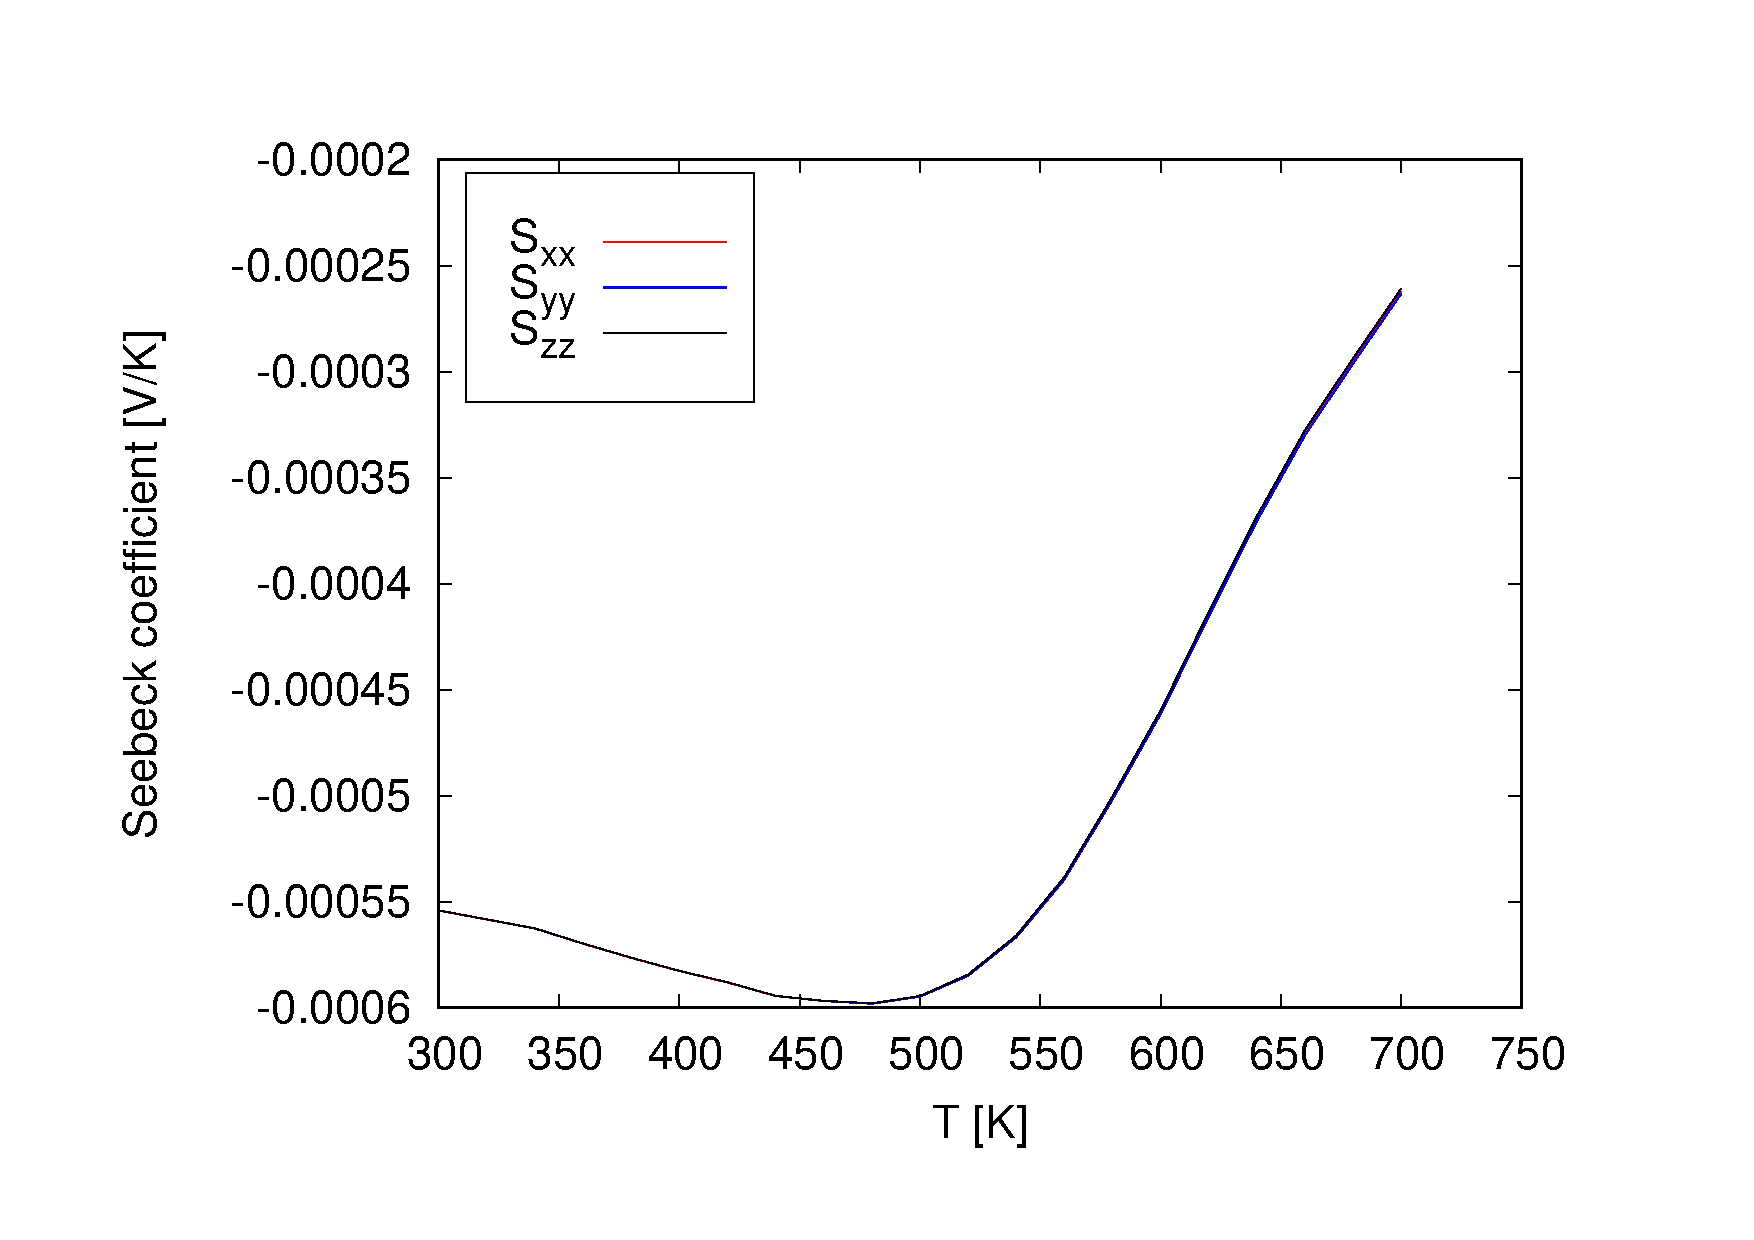
\includegraphics[width=0.7\columnwidth]{figure/example16/Si_seebeck_vs_T.pdf}
\caption{}\label{fig16.5}
\end{figure}
\end{itemize}

%\subsection*{If you do not want to use Quantum ESPRESSO}


